\section{Design and Implementation}
\label{sec:design}

The previous sections laid down theoretical foundations for root
cause analysis when complete and accurate routing information is
available. We now describe a practical system to identify the root
cause of a path change in the Internet with possibly incomplete and
inaccurate data. We now state
the goals of the system and how we achieve them.

\subsection{Goals}

Our work is motivated by the fact that Internet path changes can 
have a significant impact on performance and availability, affecting service providers, 
operators, and customers. When such changes occur, we would like to 
to be able to quickly and accurately identify the network responsible for the 
change. This allows operators to more quickly debug problems and take 
corrective action (\eg by contacting the responsible network). To enable 
such a system, we identify the following system goals.

\begin{itemize}
%
\item \emph{Accuracy:} The output candidate should include the AS that caused the change.
%
\item \emph{Precision:} The system should identify a small set of ASes 
as candidates for being the root cause of a path change, ideally a single AS or single 
AS link. 
%
\item \emph{Robustness:} The system should be able to deal reasonably
well with uncertainty or absence of information.
%
\item \emph{Scalability:} The system needs to be selective in its choice
of ASes to monitor and should introduce as little measurement overhead
as possible. It should conduct measurements and quickly identify root causes 
of path changes (\eg within minutes), enabling operators to quickly react
when an unexpected change happens.
\end{itemize}

\subsection{System Overview}

\ouralgo employs a number of measurement components
(\S\ref{subsec:measurement} and \S\ref{subsec:candidates}) to identify
the root cause of path changes observed on paths from a set of target
ASes $\mathcal{V}$ to a set of monitored prefixes $\mathcal{P}$. 
% For
%example, $\mathcal{V}$ could be the set of ASes paid to provide traffic
%to a set of prefixes $\mathcal{P}$ whose owners need accounting
%information to complain in case of performance problems; or
%$\mathcal{V}$ can be a set of ASes interested in quickly identifying
%performance problems toward a set of popular prefixes $\mathcal{P}$.
%\ic{move this to \S5 and remove it from here: ``Our current deployment targets the top 300 most common ASes on paths
%between PlanetLab nodes and toward a set of ten /24 prefixes allocated
%to the BGP-mux platform~\cite{bgpmux}.''}
As shown in \fig~\ref{fig:arch}, \ouralgo operates in two modes for each monitored prefix. In
the absence of path changes, the system stays in \emph{monitoring} mode.
The first task of monitoring mode is to estimate the set of ASes we need
to monitor to perform root cause analysis for all target ASes,
\ie $\bigcup{T(v)}$ for all $v \in \mathcal{V}$.  The second task is to
measure paths from the monitored ASes toward the monitored prefixes in~$\mathcal{P}$.  

\begin{figure}[t]
\begin{centering}
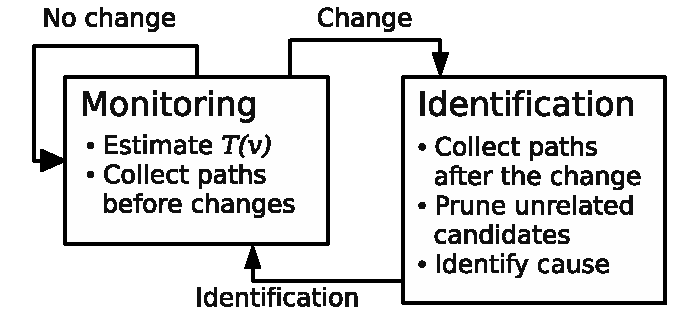
\includegraphics[width=0.9\columnwidth]{figs/arch2.pdf}
\vspace{-5mm}
\caption{\emph{PoiRoot} operation modes.}
\label{fig:arch}
\end{centering}
\vspace{.5em}
\end{figure}

\ouralgo enters \emph{identification} mode whenever the path from a
target AS $v$ to a monitored prefix changes.  Identification uses
information about the old paths used
before the change, collected while in monitoring mode.  The first step is to collect 
information about new paths used by ASes in $v$'s old path, \ie measure
$N(O(v))$. \ouralgo then runs the identification algorithm to
identify the root cause of the change.  Finally, \ouralgo returns to
monitoring mode after identification is complete.

\subsection{Path Measurement}
\label{subsec:measurement}

\ouralgo maintains an atlas of paths from each AS $v \in \mathcal{V}$
to each monitored prefix.  To this end, we combine publicly-available
BGP feeds and active traceroute measurements.  To satisfy the
assumption that there is only one routing event in the network, we need
path measurements from each AS at high enough frequency such that the
path is available before and after each routing event.  We also need to
collect all necessary information and identify the root cause before the
next routing event happens.  We describe both control- and
data-plane monitoring measurements we use below.

\nparagraph{Passive BGP Monitoring.} \ouralgo uses BGP paths made public
by over 100 RouteViews peers~\cite{routeviews}.  We download data from
RouteViews every 15 minutes.  For each monitored prefix, we store
historical and current BGP path information.  We group updates into
convergence periods if they are less than 4 minutes apart to identify
stable routes.  Previous work has shown that varying the grouping
threshold between 2 and 8 minutes has negligible impact on the resulting
convergence periods and stable paths~\cite{needle, lifeguard}.

\nparagraph{Traceroute Monitoring.}   We supplement our view of paths
toward a monitored prefix using traceroute measurements that we
translate to AS paths using IP-to-AS translation.  Specifically, every 10 minutes, 
we issue 
forward traceroutes from 175 geographically distributed PlanetLab
sites toward the monitored prefixes.  Forward
traceroutes allow us to find paths from ASes not present in route collector feeds,
but are still limited to the locations where PlanetLab nodes are located.

Reverse Traceroute~\cite{revtr} allows us to address this by potentially 
measuring paths to monitored prefixes from routers in arbitrary ASes.  In
particular, we use Reverse Traceroute to measure paths from three IPs in
each AS on the BGP feeds and forward traceroutes toward the
monitored prefixes.  We refresh reverse traceroutes every 15
minutes.  For a variety of reasons (\eg routers not responding to IP Options probes), 
Reverse Traceroute may not be able to collect
measurements from all ASes.  

\nparagraph{Combining Data Sources.}  In some cases, we obtain
a path between two ASes
using both traceroute measurements and BGP feeds. 
%Because default routes are a common
%phenomenon~\cite{optometry} and 
Because IP-to-AS
mappings can be inaccurate~\cite{as-level-traceroute, ono-sidewalk-ends}, \ouralgo uses the 
control-plane paths from BGP feeds instead of data-plane paths in this case.

\subsection{Identifying the Set of ASes to Monitor}
\label{subsec:candidates}

\ouralgo identifies the set of ASes whose paths we need to monitor to
run root cause analysis, $\bigcup{}T(v)$, while in monitoring mode. We
consider the following data sources.

\nparagraph{Passive Monitoring of Paths to Prefixes.} One way to
identify the ASes in the monitored set $T(v)$ is to continuously monitor
public BGP feeds~\cite{routeviews}.  Monitoring changes for a prolonged
period of time allows us to discover a set of paths an AS may use to
reach a prefix and build the set of ASes we need to monitor to perform
root cause analysis.  Although a passive approach reveals actual paths
used in the Internet and is minimally invasive, not all paths appear in
BGP feeds because ASes only propagate their best path, apply export
filters, and perform prefix aggregation.  Waiting for path
changes to take place naturally is likely to be slow (on the order of months or years~\cite{as-completeness}) 
for the purposes of identifying the ASes we need to monitor.

\nparagraph{Active Monitoring of Paths to Prefixes.} We complement
passive BGP data with active periodic traceroute measurements.  We store
all paths observed with passive and active monitoring and build a
database of historical paths toward the monitored prefixes.

%\nparagraph{Path Prediction.} At the other end of the spectrum is
%offline prediction of policy-compliant paths that an AS is likely to
%select when its current path to the destination becomes unavailable or
%when new paths become available.  Due to a general lack of access to an
%AS's internal routing tables, obtaining knowledge of hidden paths and
%local preferences over those paths is far from straightforward.  Using
%path prediction techniques from \emph{iPlane}~\cite{iplane}, one can
%obtain a set of paths from an AS $x$ to the destination and try to
%monitor all ASes that appear in these paths.  Although possibly
%exhaustive, we do not use this approach as it predicts a large number of
%policy compliant paths, most of which are unlikely to be ever used, and
%may lead to a prohibitively large set of ASes to monitor.\ic{We don't
%use this; candidate for removal.}

\nparagraph{Revealing Alternative Paths via BGP Announcements.} \ouralgo
reveals alternative paths in the Internet using the Transit Portal
platform~\cite{bgpmux}, which lets us announce prefixes using five
different US universities as our providers (University of Washington,
University of Wisconsin, Georgia Tech, Princeton University, and Clemson
University).  Suppose AS $v$ has AS $x$ in its path toward a prefix we
control in AS $s$.  To reveal an alternative path from $v$ to
$s$ that does not traverse $x$, we can prepend our BGP announcements
with $[s, x, s]$.  This approach is generally referred to as 
``BGP poisoning''~\cite{optometry, lorenzo-thesis, lifeguard}.\footnote{Similar to 
the study we conducted for LIFEGUARD~\cite{lifeguard}, these announcements 
affect only paths toward our experimental prefixes and we impose a conservative 
rate limit for announcements to ensure our experiments do not generate unduly 
large numbers of updates. We gave operators an opportunity to opt out.
We have received zero complaints during several 
months of experiments.} 

When a poisoned update for our prefix arrives at $x$,
BGP's loop-prevention mechanism causes $x$ to discard the route, leaving it routeless.
AS $x$ then withdraws its path to our prefix
from its upstream neighbors (including $v$), forcing them to choose new
paths.  For example, in \fig~\ref{fig:induced3} poisoning $c$ emulates a
link failure between $c$ and $b$.  This causes $c$ to withdraw the route
to $b$, causing $b$ to route through $d$.  

%Poisoning emulates a change in link availability and hence forces a path
%change.  It is a middle ground between monitoring of path changes ``in
%the wild'' and simulating policy-compliant paths.  

% By systematically and cumulatively poisoning ASes in the paths used by
% AS $x$ to reach $d$, we can discover paths from $x$ to $s$.  Also, we
% can infer local preferences at $x$ by looking at the order in which
% $x$ picks paths as we poison ASes.

To discover all possible paths to our prefixes from an AS $x$, we first
discover all neighbors $L(x)$ that $x$ can use to reach our prefix and
then call the discovery process recursively on each AS in $L(x)$.  To
discover the neighbors $L(x)$ that an AS $x$ can use, we first poison
the neighbor $O_\mathrm{n}(x)$ that $x$ is using to reach our prefix.
When $x$ changes to a new path, we poison its new neighbor.  
We repeat this process until $x$ has no new path to our prefix.
Note that we include multiple ASes in our announcements as the discovery process
proceeds. In particular, to call the discovery process recursively on an
AS $y \in L(x)$, we need to poison all other ASes in $L(x)$ that $x$
prefers over $y$.  For example, suppose our measurements go through a
provider $x$ that has $y$ and $z$ as the two most preferred neighbors to
reach our prefixes. We will keep $y$ poisoned throughout the discovery
of the paths $z$ can use toward our prefixes, otherwise $x$ would change
back to $y$ and we will be unable to observe paths through $z$.  

We argue that this approach to learning alternative available paths is
reasonable for the context of a large cloud provider or ISP. Such
networks already are BGP speakers, and we expect they can dedicate a
small prefix (\eg a /24) for the purposes of exploring alternate paths and
inferring route preferences of different ISPs routing towards them.

\nparagraph{Path Preference Estimation.} We use the order in which $x$
chooses neighbors in the path discovery procedure above to rank paths by
preference.  When the discovery procedure provides insufficient
information to estimate preference, we use path usage time as in
indicative of preference as proposed by Oliveira \emph{et
al.}~\cite{oliveira09exploration}.


% If an AS $d$ that originates a prefix wants to discover alternative
% paths that another AS $x$ has to its prefix, it can choose $x$'s next
% hop (or another downstream AS), say $O_\mathrm{n}(x)$, and prepend
% that AS in its announcement for that prefix.  When $O_\mathrm{n}(x)$
% receives the prepended announcements, it rejects the route due to BGP
% loop detection.  This, in turn, forces $x$ to use the next best route
% available toward $s$.


\subsection{Root Cause Analysis Algorithm}

The root cause analysis algorithm in Alg.~\ref{algo:rules} requires
complete and accurate information. \ouralgo uses a modified version,
shown in Alg.~\ref{algo:practical}, that is more robust to missing and
inconsistent measurements. Because it is impossible to determine
whether an AS changed its export policy without BGP feeds from its
neighbors, we assume that ASes do not change their export policy (\ie unless 
an AS changes its path, it will not change whether or not it is exporting the path to a neighbor). 
If an AS
changes its export policy in practice, our system will blame the root
cause's upstream. We believe this case is uncommon. Further, 
this information is useful in that the upstream AS is the only one 
that could detect the change in export policy, information necessary 
to debug the path change.

We now describe how our practical root cause analysis algorithm works.
Suppose a path change happens on the path from an AS~$v$ to another AS
$s$ that originates a prefix.  The algorithm adds the ASes in $O(v)$ and
$N(v)$ to the suspect set $\mathcal{S}$.  At each step, the algorithm
visits the unvisited AS $x$ in the suspect set that is closest to $v$
(ties can be broken arbitrarily).  If a
measurement from $x$ is missing (lines~3--4), the algorithm uses several
heuristics to resolve uncertainty, described in
\S\ref{subsec:uncertainty}.  If the visited AS $x$ did not change paths,
then $x$ cannot be the root cause and we remove $x$ and all downstream
ASes from the suspect set (\localC{}, lines 5--7).  If $x$ changed
paths, we know that either it is the root cause or the root cause is
downstream of~$x$ (\neighborC{} or \downstreamC{}).  We remove all ASes
upstream of $x$ from the suspect set (line~9).  If $x$ is in $O(v)$ or
$N(v)$, then we add any new ASes downstream of $x$ to the suspect set
and visit them to determine whether they are the root cause of the path
change.  Note that this algorithm has no recursive call and that
lines~11 and~13 only execute if $x \in O(v)$ or $x \in N(v)$.  Only ASes
in $N(O(v)) \cup O(N(v))$ may be added to the suspect set.  The
algorithm finishes when all ASes in the suspect set have been visited.
\looseness=-1

Our algorithm will misidentify the root cause if our simplified routing
model is wrong; \ie the root cause AS is not in $N(O(v)) \cup O(N(v))$.
Say Alg.~\ref{algo:practical} identified $x$ as the root cause.  We can
check for violations of the model (and misidentifications) by extending
Alg.~\ref{algo:practical} to check if another downstream AS in $O(x)
\cup N(x)$ changed paths.  Our algorithm further assumes there is a
unique path change when performing root cause analysis.  For concurrent
changes where the root causes are in one AS (or at an AS-AS boundary),
\ouralgo will correctly identify the AS responsible.  \ouralgo is
equally effective when concurrent changes affect disjoint sets of paths.
The case of distant, unrelated concurrent changes may lead to
misidentifications (\eg identifying multiple, incorrect root causes).

% Our algorithm cannot identify the root cause of path change if our
% model is wrong; \ie the root cause AS is not in $N(O(v))$ or
% $O(N(v))$.  In this case, the path change would reveal an AS $a$ not
% in the monitored set. To address this problem, our algorithm will add
% $a$ to the suspect set and flag the suspect set as potentially
% incomplete.

% This is because in the former case, if we have $O(x)=N(x)$ for AS $x$,
% Rule~3 from \S\ref{subsec:rules} allows us to eliminate all of $x$'s
% successors from consideration. On the other hand traversal by order of
% prefix propagation will require checking each of $x$'s successors in
% turn to achieve the same result.\ic{I prefer the explanation `in order
% of propagation from s' myself; anyway, I think we can just choose one
% order and don't need to talk about the other}

\begin{pseudocode}[t]
\textbf{PracticalRootCause(v, s):}\\
%
{\scriptsize 1}\hspace*{1em}$\mathcal{S} \leftarrow O(v) \cup N(v)$\\
{\scriptsize 2}\hspace*{1em}\textbf{for each} unvisited $x \in 
\mathcal{S}$ in order of distance from $v$:\\
%
{\scriptsize 3}\hspace*{2em}\textbf{if} $O(x)$ not found \textbf{or}
$N(x)$ not found\textbf{:} \\
{\scriptsize 4}\hspace*{4em}// resolve uncertainty (\S\ref{subsec:uncertainty})\\
%
{\scriptsize 5}\hspace*{2em}\textbf{if} $O(x) = N(x)$\textbf{:} \\
{\scriptsize 6}\hspace*{4em}remove $x$ from $\mathcal{S}$ \\
{\scriptsize 7}\hspace*{4em}remove ASes downstream of $x$ from $\mathcal{S}$ \\
%
{\scriptsize 8}\hspace*{2em}\textbf{else:} \\
{\scriptsize 9}\hspace*{4em}remove ASes upstream of $x$ from $\mathcal{S}$\\
{\scriptsize 10}\hspace*{3.7em}\textbf{if} $x \in O(v)$\textbf{:}  \\
{\scriptsize 11}\hspace*{5.7em}add ASes in $N(x) - O(x)$ to $\mathcal{S}$ \\
{\scriptsize 12}\hspace*{3.7em}\textbf{else if} $x \in N(v)$\textbf{:} \\
{\scriptsize 13}\hspace*{5.7em}add ASes in $O(x) - N(x)$ to $\mathcal{S}$\\
{\scriptsize 14}\hspace*{0.7em}\textbf{return} $\mathcal{S}$
%
\caption{Practical algorithm for root cause analysis of a change on the
path from $v$ to $s$ with potentially incomplete information.}
\label{algo:practical}
\end{pseudocode}

\subsection{Dealing with Uncertainty}
\label{subsec:uncertainty}

Alg.~\ref{algo:practical} can find the root cause of a path change
using a small subset of all monitored ASes in $T(v)$.  However,
some path measurements might be unavailable.  In particular,
measurements for the new path of an AS $x \in O(v)$ may be unavailable 
because no vantage point has a path that traverses $x$ after the change.
Similarly, measurements for the old path of an AS $y \in N(v)$ may be
missing.  We employ the following heuristics to deal with missing
measurements in Alg.~\ref{algo:practical}.

\nparagraph{FailedPath.}  If AS $x$ experiences an outage, \ie $O(x) \ne
N(x)$ and $N(x) = \emptyset$, then the root cause is downstream of $x$
and all ASes upstream of $x$ cannot be the root cause (\localC{} or
\neighborC{}) and we remove ASes upstream of $x$ from the suspect set.
Similarly, \textbf{FailedPath} removes $x$'s upstream ASes in the case
of a link restoration, \ie $N(x) \ne O(x) = \emptyset$.  We keep track
of reachability from ASes using pings to historically reachable routers
inside ASes.

\nparagraph{MissingPath.} If a path from AS $x$ is unavailable and $x$
is reachable, we use information from our atlas of historical paths
(\S\ref{subsec:candidates}) to predict the missing path.  When either
$O(x)$ or $N(x)$ is missing, \textbf{MissingPath} adds all ASes in $x$'s
bounded monitored set, $T(x)$, to the suspect set, as these are the ASes
that $x$ is most likely to be using after the change.

\vspace{0.4em}
%
\nparagraph{Correlation.} When Alg.~\ref{algo:practical} runs and 
encounters missing measurements, the resulting candidate sets may
contain more than one AS.  Because routing is generally destination-based, 
the same root cause can appear in multiple paths from vantage points toward 
the monitored prefix. We use this observation to reduce the suspect set by correlating
suspect sets across path changes from the same event observed at
different vantage points. 

Note that the candidate sets from different vantage points may be
disjoint for two reasons. First, our information about routing
preferences for each AS in the candidate set may be incorrect (\eg
because it is stale) leading the system to monitor the wrong set $T(v)$
of ASes. Second, there may be multiple concurrent and independent path
changes.  Thus, taking the intersection of suspect sets, as done by
Feldmann \etal~\cite{feldman}, would filter out a potential root cause. 

To avoid this, we compute the suspect set for each path change resulting
from a network event, then count the number of occurrences of each
suspect AS over all suspect sets.  Then, each suspect set is pruned to
only those ASes with the highest number of occurrences.

\begin{comment}
\begin{algorithm}{Root Cause}
\label{algo}
\begin{algorithmic}
%\COMMENT{Build the initial suspect set} \\
\hrule
\item[]
\REQUIRE{vantage point $V$, old path $O(V)$, new path $N(V)$, time indexed by $t$, 
path directory \texttt{path} where \texttt{path[A][t]} is A's path at time $t$}
\ENSURE{Suspect Set \textbf{\emph{SS}}}
\hrule
\item[]
\STATE  \textbf{\emph{SS}} $\leftarrow \{\}$
\FOR{$A$ in $O(V)$}
\STATE add $A$ to \textbf{\emph{SS}}
\ENDFOR
\FOR{$A$ in $N(V)$}
\STATE add $A$ to \textbf{\emph{SS}}
\ENDFOR
\item[]
\FOR{$A \in$ \textbf{\emph{SS}} in order of prefix propagation}
\STATE $O(A) \leftarrow \texttt{path[A][t-1]}$
\STATE $N(A) \leftarrow$ \texttt{path[A][t]}
\IF{$O(A)$ not found \textbf{or} $N(A)$ not found}
\STATE \texttt{Uncertainty(\textbf{\emph{SS}})}
\ELSIF{$O(A) \equiv N(A)$}
\STATE remove $A$ from $SS$
\STATE \textbf{continue}
\ELSIF{$O(A) \not \equiv N(A)$}
\STATE \IF{$A \in O(V)$}
       \STATE \texttt{New\_ASes} $\leftarrow \{N(A)-O(A)\}$
       \FOR{$B$ in \texttt{New\_ASes}}
       \STATE add $B$ to \textbf{\emph{SS}}
       \ENDFOR
       \STATE let $O(V) \leftarrow \{V,\dots,B,A,\dots,S\}$
       \STATE remove \{V,\dots,B\} from \textbf{\emph{SS}}
       \ELSIF{$A \in N(V)$}
       \STATE \texttt{New\_ASes} $\leftarrow \{O(A)-N(A)\}$
       \FOR{$B$ in \texttt{New\_ASes}}
       \STATE add $B$ to \textbf{\emph{SS}}
       \ENDFOR
       \STATE let $N(V) \leftarrow \{V,\dots,B,A,\dots,S\}$
       \STATE remove \{V,\dots,B\} from \textbf{\emph{SS}}
       \ENDIF
\ENDIF
\ENDFOR
\item[] \hrule \item[] \hrule
\STATE\hspace{-0.1in}\textbf{Uncertainty}
\hrule
\REQUIRE{Suspect Set \textbf{\emph{SS}}, AS $A$, old path from vantage point $V$ $O(V)$, new path $N(V)$}
\ENSURE{Suspect Set \textbf{\emph{SS}}}
\hrule
\IF{$A$ is not reachable}
   \IF{$A \in O(V)$}
   \STATE let $O(V) \leftarrow \{V,\dots,B,A,\dots,S\}$
   \STATE remove \{V,\dots,B\} from \textbf{\emph{SS}}
   \ELSIF{$A \in N(V)$}
   \STATE let $N(V) \leftarrow \{V,\dots,B,A,\dots,S\}$
   \STATE remove \{V,\dots,B\} from \textbf{\emph{SS}}
   \ENDIF
\ENDIF
\end{algorithmic}
\end{algorithm}


\begin{pseudocode}
\textbf{Given:} vantage point AS $V$, time $t$,
path directory \texttt{path} \\
\hrule 
\hspace{1in}
\\
\textbf{GetPath} \\
$p \leftarrow$ \texttt{path[V][t]} \\
if $p$ exists \\
    \hspace*{0.1in} return $p$ \\
{// when $p$ doesn't exist, there is either no path or path measurement is unavailable} \\
{// check pingability} \\
if $V$ is \textbf{unreachable} \\
    \hspace*{0.1in} return $[]$ \\
(// at this point we have established that  $V$ has a path back) \\
%$p_f$ \leftarrow \texttt{traceroute(V)} \\
\textbf{for each} historical neighbor AS $X$ of V  \\
   \hspace*{0.1in} $q_x$ \leftarrow \texttt{path[X][t]} \\

{//pick the right $q_x$ somehow} \\
   
   return \emptyset
    
\caption{Algorithm}
\label{fig:rca-algo}
\end{pseudocode}
\end{comment}
